\chapter{Предлог решења} \label{ModelProposal}
\section{Android}
Све функционалности које би се желеле у претходној глави требале би на неки начин да се испуне. Први проблем је организација Android дела и које ће све могуће активности бити. Предлог је да их буде пет : почетна, резултати, подешавања, игра, уређивање.
\begin{figure}[htb!]
\begin{center}
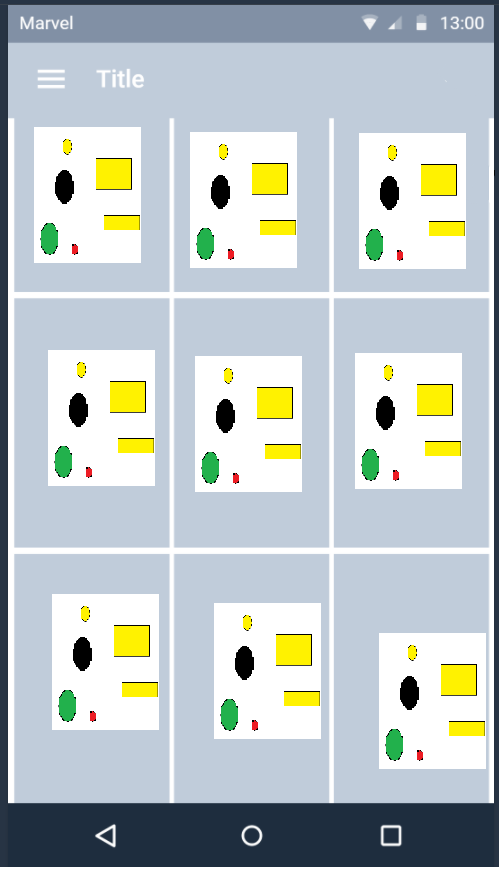
\includegraphics[scale=.5]{pictures/prototype/mainActivity}
\caption{Прототип почетне активности}\label{fig:prototypeBeginActivity}
\end{center}

\end{figure}

 Из почетне активности (слика \ref{fig:prototypeBeginActivity}) корисник бирањем опције из главног менија прелази на уређивање, игру или подешавање. Имао би листу свих полигона из које би кратиким притиском прста прелазио на играње одговарајућег полигона. Задржавањем притиска прста на некој од њих би му искочио падајући мени из кога би бирао да ли би желео да обрише или да уређује тај полигон. Бирањем уређивања прешао би на активност уређивање. 

\begin{figure}[htb!]
\begin{center}
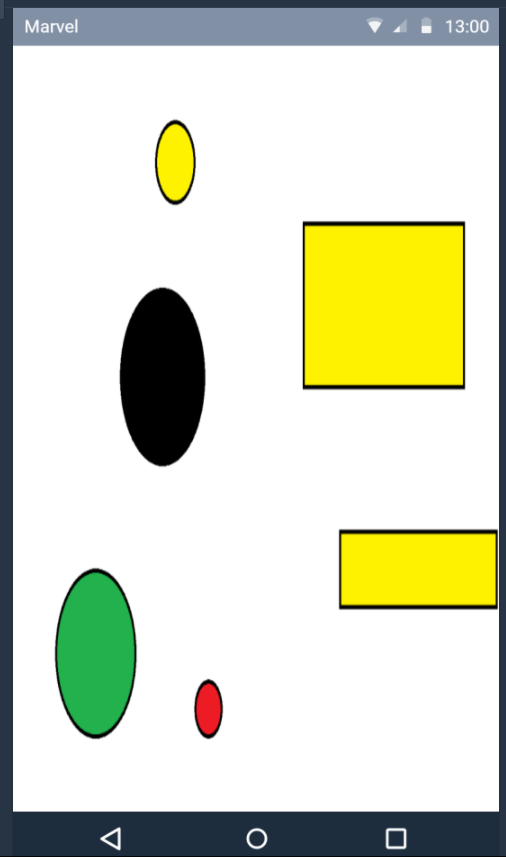
\includegraphics[scale=.5]{pictures/prototype/gameActivity}
\caption{Прототип игре}\label{fig:prototypeGameActivity}
\end{center}
\end{figure}

Сама игра (слика \ref{fig:prototypeGameActivity}) би му нудила препреке одговарајуће боје које би му указивале на то ког су типа, да ли се одбија од њих. да ли може да улети у њих и слично. У њему би била примењена физика чији прототип је у поглављу \ref{Collision}. Кад корисник упадне у препреку у коју не сме, био би крај игре. У случају успеха (стизања до краја), кориснику би се понудило да се упише на листи и био би пребачен на резултате за тај  полигон. 

\begin{figure}[htb!]
\begin{center}
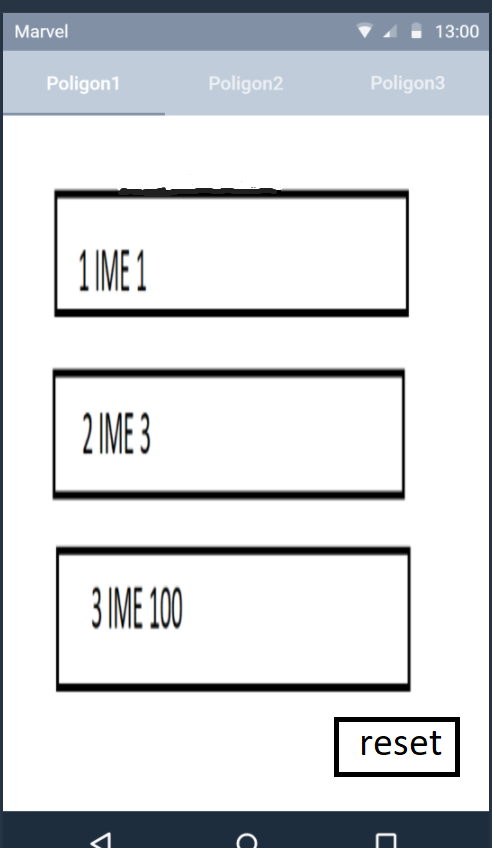
\includegraphics[scale=.5]{pictures/prototype/resultsActivity}
\caption{Прототип резултата}\label{fig:prototypeResults}
\end{center}
\end{figure}

Активност резултати (слика \ref{fig:prototypeResults}) би приказивала листу свих резултата за тај полигон са редним бројем резултата, имену и скору. Поред тога корисник би имао могућност да види резултате различитих полигона. Било би могуће и ресетовати резултате за дати полигон.

\begin{figure}[htb!]
\begin{center}
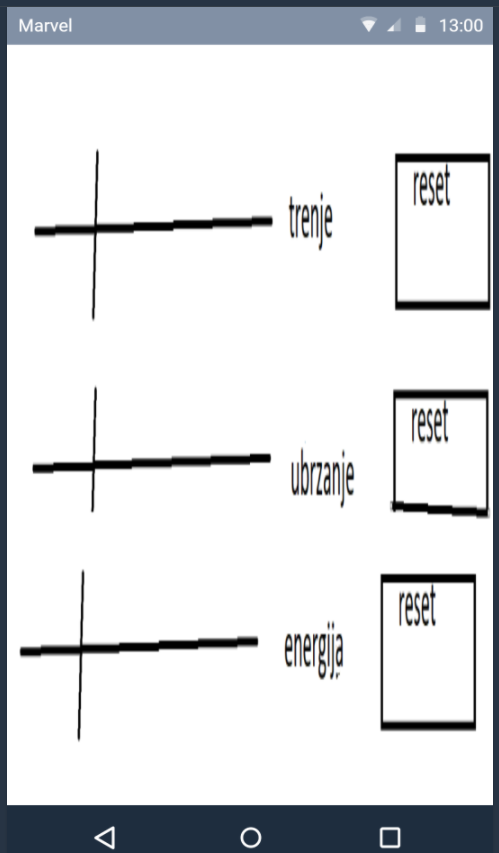
\includegraphics[scale=.5]{pictures/prototype/settingsActivity}
\caption{Прототип подешавања}\label{fig:prototypeSettings}
\end{center}
\end{figure}

Активност подешавања (слика \ref{fig:prototypeSettings}) дозволила би кориснику да подешава параметре који се користе током играња игре. Од параметара би се користили коефицијент трења, коефицијент убрзања,  и проценат губитка брзине приликом судара са препреком која није кобна по лопту. Такође било би могуће вратити подешавања за сваки параметар на почетни одговарајућим дугметом.

\begin{figure}[htb!]
\begin{center}
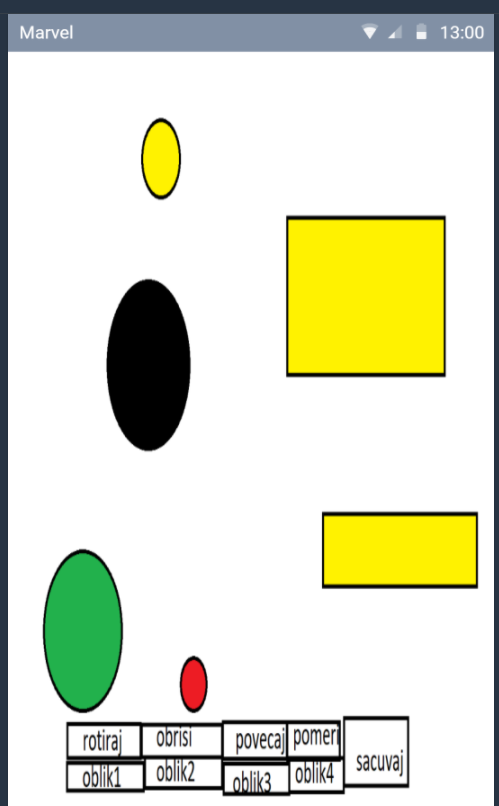
\includegraphics[scale=.5]{pictures/prototype/createPolygonActivity}
\caption{Прототип уређивање полигона}\label{fig:createPolygonActivity}
\end{center}
\end{figure}

Активост уређивање (слика \ref{fig:createPolygonActivity}) дозволила би кориснику додавање новог или уређивање постојећег полигона. Код сваког уређивање (новог или постојећег) корисник би имао опције да ротира одговарајући објекат, да га помери, да му промени величину, или да га обрише. Поред тога имао би могућност да дода нове објекте (почетну позицију лопте, крајњу рупу у коју лопта треба да се убаци, вртлог, амбис, правоугаону препреку, кружну). Након рада корисник би имао могућност да одговарајућим дугметом сачува полигон.

\section{Развојно окружење}
За прорамски језик биће коришћена Java, искључиво, јер омогућава лакшу израду пројекта и лакше дебаговање. У комбинацији са Java биће коришћeн xml за израду GUI\footnote{Graphical User Interface}. Биће коришћен  Android Studio\footnote{\url{https://developer.android.com/studio/index.html}} који ће давати лагодност у погледу дебаговања, build-овања и праћења промена. Он омогућава интегрисани рад са системима за праћење ревизија попут Git (линк \cite{BitBucket}). У наставку се налази списак свих алата који ће бити коришћени:
\begin{table}[H]\centering
\begin{tabular}{ l  l } \toprule
{\bf Алат} & {\bf Сврха}\\ \midrule
{\tt AndroidStudio 2.3.3} & IDE\\
{\tt compileSdkVersion 25.0.1} & систем за build-овање уграђен у AndroidStudio\\
{\tt SourceTree 2.1.2.5.} & Систем за ревизију\\
\TeX Maker 4.5 & \LaTeX\ уређивач\\
\bottomrule
\end{tabular}
\caption{Алати коришћени при развоју пројекта.} \label{UsedTools}
\end{table}
Машина на којој ће бити писан и компајлиран код и на којој ће радити Android Studio је HP Omen са 12GB RAM, 512GB SSD, i7-6700HQ 2,7GHz, оперативни систем Windows 10.0.15063. Машина на којој ће бити покретана апликација је NVIDIA Shield Tablet K1, који је у тренутку првог инсталирања имао Android 5.0 верзију инсталирану. \footnote{У тренутку писања последњих измена ажуриран је на Android 7.0}. Минимални Андроид ОС\footnote{Оперативни систем} који подржава апликацију је 5.0.

\section{Модел физике} \label{Collision}

Модел физике биће имплементиран у оквиру једне класе засад је назовимо \emph{CollisionModel}. Књига која ће бити коришћена за упрошћен модел физике је \cite{EngBook}. Поред тога биће коришћен и увид у код који иде уз њу, који се налази на линку адресе у референци \cite{ModCol}.
\\ \indent
Прво са сензора се детектује ново убрзање које делује на уређај (гравитационо + убрзање уређаја) и оно се филтрира да би се спречиле превелике осцилације у убрзању. Разлог за филтрирање је ако сензор нешто погрешно прочита. Даље филтрирано убрзање као и време кад је детектовано прослђује се моделу са листом фигура и лоптом (позиција, полупречник). Ово је опис система до "предаје" управљања лопте класи \emph{CollisionModel}.
Даље се убрзање скалира (множи са одговарајућим коефицијентом из подешавања апликације) што омогућава да лопта пуно брже реагује на промене убрзања уређаја.
Даље, лопта у сваком тренутку има вектор кретања брзине по све три осе $v_x, v_y, v_z$. Да би се израчунале нове брзине $v_x, v_y$ потребно је "потпуно" убрзање (сила) која делује на лопту. "Потпуно" убрзање се рачуна тако што се скалирано убрзање потом дода на трење (боље речено одузме). Трење се рачуна као убрзање по $z$ оси скалирано са коефицијентом трења добијеним из подешавања апликације, али тако да има знак супротан од брзине. Овај модел трења је реалистичан јер трење и у стварности је $\mu N$, где је $N$ нормална сила (на уређају је убрзање у суштини та нормална сила). Потом се нова брзина рачуна
$$v_i=v_{previousi} + a_{full}  \Delta T, i \in \{x, y\}$$
При чему је $a_{full}$ "потпуно" убрзање, $v_{previousi}$ претходна брзина лопте, а $v_i$ нова и $\Delta T$  разлика између времена претходне детекције сензора и тренутне детекције (који се обрађује). Ако је брзина променила смер по некој од оса и трење је утицало на то, брзина по тој оси постаје 0.
\\ \indent
Сад се рачунају потенцијалне нове позиције лопте по формули:
$$i = i_{old} + v_i \Delta T, i\in{x, y}$$
Где је $i$ нова координата центра лопте по одговарајућој оси, а $i_{old}$ стара координата. Потом се рачунају судари са свим фигурама на екрану И за оне фигуре са којима се сударила рачуна се како утичу на промену брзине. Све те фигуре утичу на промену брзине.  Постоје два типа фигура.
\\ \indent
\begin{figure}[htb!]
\begin{center}
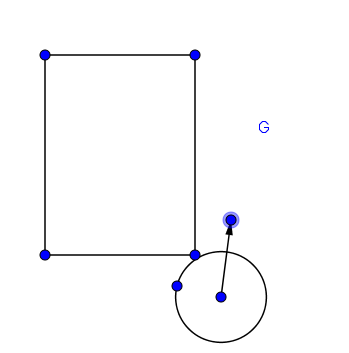
\includegraphics[scale=.5]{pictures/physics/ballRectDown}
\caption{Судар лопте и правоугаоника кад се лопта креће нагоре}\label{fig:ballRectDown}
\end{center}
\end{figure}
\begin{figure}[htb!]
\begin{center}
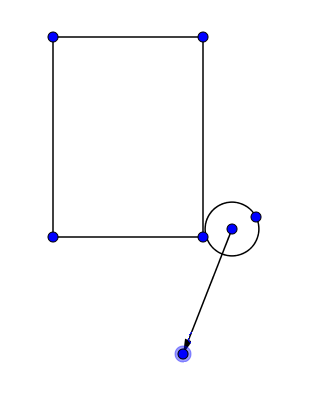
\includegraphics[scale=.5]{pictures/physics/ballRectUp}
\caption{Судар лопте и правоугаоника кад се лопта креће надоле}\label{fig:ballRectUp}
\end{center}
\end{figure}

Први су класичне препреке од које лопта одбија. Могу бити правоугаоне (квадрасте) или кружне (лоптасте).
За правоугаонке је коришћен упрошћен модел, где су странице правоугаоника паралелне осама.
Промена брзине рачуна тако да под оним углом којим је ушла мора да се и одбије (за случај кад удара само страницу правоугаоника, без ћошка).То је одрађено простом провером гледа се у коју страницу удари и онда ако је ударила у страницу чија је оса паралелна рецимо оси $x$ онда се мења брзина $y$ (враћа се негативна вредност по тој оси). Аналогно и за осу $y$.  Док кад удари ћошак врши се промена брзине по оси као у случајевима да није ћошак, али само под условом да се "приближава" тој ивици. Кад се каже приближава, мисли се у случају кад рецимо лопта прилази са доњој страници правоугаоника са доње стране, онда ће се "одбити" по $y$ оси (слика \ref{fig:ballRectDown}). Али у случају кад би прилазила са горње стране не би се одбила по $y$ оси (слика \ref{fig:ballRectUp}).   Ово спречава да се лопта "заглави" на ћошку, а и даје релативно реалистичан судар. Кад се ради са правоугаоницима којима странице нису паралелне осама, проблем се сведе на претходни. Изврши се проста ротација читавог координатног система (уједно и брзине лопте) за угао $-\alpha$ при чему је $\alpha$ угао под којим се налази правоугаоник у односу на $x$ осу. Ротација се врши множењем сваке координате коју смо користили у старом систему ротационом матрицом \footnote{\url{http://mathworld.wolfram.com/RotationMatrix.html}}. Тако да је нови проблем сведен на већ решен. Проблем се реши као у претходном случају и онда се промена брзине само врати у почетни систем ротацијом промена брзине за $\alpha$. Пошто ротација захтева рачунање $\sin$ и $\cos$ биће коришћене оптимизације по којој су они израчунати унапред (кад се учитава полигон) и онда нема губитка времена при њиховом израчунавању.
\\ \indent
За кружне препреке тражена брзина је :
$$v_{new} = v_i - 2 \frac{\langle v_{old}, c_1 - c_2 \rangle (c_1 - c_2)}{||c_1-c_2 ||^2 }$$
При чему су $c_1$ стара координата центра лопте (пре потенцијалног померања), $c_2$ координата центра препреке са којом се лопта судара, $v_{old}$ брзина лопте као и $v_{new}$ брзина која треба да се добије. При чему је $|| nesto||$ ознака за дужину вектора, док је $\langle n_1, n_2 \rangle$ ознака за скаларни производ два вектора $nesto_1, nesto_2$. Промена брзине се рачуна:
$$v_{change} = \frac{v_{new} - v_{old}}{2}$$
Овај начин рачунања избегава било какво коришћење тригонометрије и због тога је брз.
\\ \indent
Друга врста препрека су рупе.
Има их три типа (крајња рупа, амбис, вртложна рупа), али у суштини се све три понашају на исти начин. Све покушавају да привуку лопту у себе, при чему амбис и крајња рупа завршавају игру, док кад упадне у вртлог игра даље траје.
Промена брзине се рачуна по формули:
$$v_{change} =  \frac{(c_2 - c_1) \cdot GRAVITY\_CON}{|| c_2-c_1||^2}$$
Овде су $c_2$ нова координата лопте, $c_1$ координата препреке. Док је $GRAVITY\_CON$ константа којом се лопта привлачи.
\\ \indent
Након што се израчунају промене брзине за све сударе у том тренутку лопте, оне се множе са 2 и све се сабирају. Након тога ако нема промене брзине по $x$ координати или је лопти промењена брзина под утицајем рупа лопта може да се помери на новоизрачунату координату по тој оси. Иначе по $x$ оси не може. Аналогно је и за $y$ осу. На крају брзина се мења додавањем збира промена брзине по тој оси на брзину генерисану након рачунања "потпуног" убрзања. Под условом да је брзина промене различита од 0 или под условом да се лопта "сударила" са рупом претходно израчуната брзина губи одређен проценат који је подешен у подешавањима апликације.

\section{Модел графике}
Док ће се за активности у којима није потребно учестало исцртавања екрана бити коришћена GUI нит, тамо где је потребно (активност игра, уређивање) мора се наћи другачије решење. За површ уместо стандардног \emph{Canvas}-a који припада \emph{ImageView}, који захтева исцртавање целог екрана \footnote{\url{https://developer.android.com/reference/android/widget/ImageView.html}} користиће се \emph{SurfaceView} који се само освежи (остатак екрана се не мења) кад је неопходно. И то исцртавање радиће се у посебној нити, која кад заврши посао, само ће заменити \emph{Canvas}  SurfaceView-ов canvas са новим Canvas-ом. Што умањује заузетост GUI нити непотребним рендеровањем, и омогућава да се користи у рачунању и ажурирању SurfaceView-а.
Ради смањења загревања уређаја, нова нит која исцртава \emph{Canvas} то ће радити само кад је затражено од ње (кад се десила промена позиције), остатак времена спава. 
